\section{Latent Variable Models}

\thispagestyle{empty}
Latent variable models have been a cornerstone of complex, high dimensional data analysis for a long time. They are slightly different from the methods mentioned earlier in the sense that here one tries to understand the underlying data structure by assuming that the observations are a result of interaction between an unknown number of hidden or latent variables (Raiko et al., 2006) and hence the objective is to learn both the hidden variables and the interaction or process.

The latent representations learnt during data analysis can be very task specific for example, in order to reduce dimensionality these learned representations can summarise the most relevant aspects of high dimensional data in fewer dimensions or can aid in recognizing patterns by extracting important non measurable aspects or features from data. Thus latent variable models provide a simple flexible framework under which various different statistical methods can be unified (Bartholomew, Knott, & Moustaki, 2011).  

If we consider latent variable as the parameters of data, the idea of learning hidden variables and the process through which they generate observations closely follows the Bayesian inference process described in section 1 and inverse of generation process can also be referred as projection of data to latent space. This interaction between latent variables or mapping to latent space can be linear or non-linear. Linear interactions like FA, PCA, ICA [hyvornen et al?] etc, though interpretable due to their simplicity and computationally fast, may not be suitably in cases where a complex latent space mapping is to be found. Non linear interactions on the other hand can provide enough capacity to model complicated processes at the cost of interpretability and computational ease. Self organizing maps [Karhunen], non linear PCA[Valpola 2004], Gaussian process latent vector model [], non linear space mdoels [Valpola 2005] are some of the examples of non linear LVMs.

In the following subsections we first describe the foundational linear model called Factor Analysis froma probabilsitic perspective and then move on to a more sophisticated latent model called GP based FA. 

\subsection{Probabilistic Factor Analysis}
Originated from in psychological research in early 19th century, Factor models are considered one of the oldest linear latent variable methods (Bartholomew et al., 2011). It derives its name from two factor model presented by (Spearman, 1904) postulating that test scores of individuals can be thought of as linear combinations of two factors, namely common factor- akin to one’s general intelligence and another specific to the context of test (Anderson & Rubin, 1956). 

Central objective behind factor analysis is to describe the co-variance among large number of observed variables in terms of less number of underlying latent variables, called factors. This ability to explain away the variation can also enable factors to express commonalities hidden in data, making them very suitable tool for extrapolatory data analysis.

Consider an observed data set ${Y \in N \times P}$ and factors ${X \in N \times Q}$, where commonly ${Q << P}$. According to traditional FA model(Anderson & Rubin, 1956; Bartholomew et al., 2011), each instance of Y is assumed to be generated by a linear transformation of uncorrelated factors X such that , 
\begin{equation}
Y_i = \Phi X_i + \mu + E_i, 
\end{equation}

Where, ${\Phi}$ is a constant matrix representing the linear transformation of factors X. Values of ${\Phi}$ correspond the amount of influence a particular factor has on the observed data and thus are appropriately named as factor loadings, ${\mu}$ is the mean vector. Factors ${X_i}$ as well as noise ${E_i}$ are assumed to be Gaussian distributed as ${\mathcal{N}(X_i| 0, I)}$ and ${\mathcal{N}(E_i | 0,\Psi)}$ respectively. 

This gives us a normally distributed generative model of data given by,
\begin{equation}
Y_i \in \mathcal{N}(Y_i | \mu,  \Phi\Phi^T + \Psi)
\end{equation}

It can be observed that if ${\Psi}$ is a diagonal matrix estimated from observations, covariance in Y can be solely explained by the latent factors while ${E_i}$ models the individual variability of each data instance ${Y_i}$. A detailed review of various properties of FA models can be found in (Bartholomew et al., 2011).

Due to its popularity, a number of inference methods both Bayesian and non Bayesian have been proposed to estimate FA parameters over time (Anderson & Rubin, 1956; Jöreskog, 1967; Lawley, 1940; Press & Shigemasu, 1989; Rowe, Rowe, & Press, 1998; Rubin & Thayer, 1982). In addition to the ability of including prior or expert knowledge about factors, Bayesian approaches have added consequence of eliminating rotational ambiguity in estimation of factor loadings.

In Bayesian formulation of Factor analysis, we put a prior over factor loading matrix ${\Phi}$ and substitute error covariance matrix ${\Psi}$ with its inverse, precision matrix ${\psi}$.
\begin{equation}
p(\Phi) = \prod_{q=1}^{Q} \mathcal{N}(\phi_q | 0, f_q^{-1}I)
\end{equation}
\begin{equation}
p(f) = \prod_{q=1}^{Q} \mathcal{G}(f_q | a_{q}^{f}, a_{q}^{f})
\end{equation}
\begin{equation}
 p(\psi) =  \mathcal{G}(\psi | a^{\psi}, b^{\psi}) \hspace{1em}, \psi = \Psi^{-1}.
\end{equation}

Here, ${\phi_k}$ represents kth column of the loading matrix (or kth factor) which is isotropically Gaussian distributed with the precision matrix represented by ${f_k}$.Precision matrices ${\psi}$ and ${f_k}$ are given Gamma priors controlled by their respective hyper-parameters. Being the precision of zero mean Gaussian, ${f_k}$  can be used to shut off corresponding redundant factors.

Joint posterior distribution of parameters ${p(\Phi, X, \mu, \psi, f | Y )}$  is analytically intractable and must be approximated. (Ghahramani \& Beal, 2000; Nielsen, 2004) provide detailed derivations for variational inference over a fully factorized approximated distributions of this posterior. However, these methods are known to have some downsides like heavier penalization of model or inability of solution to shut down redundant factors specially in observations with minimal noise which was more recently overcome by (Zhao & Yu, 2009) in their improved VB schemes.

Distributional assumptions of factors and noise terms in FA are of utmost importance since slight variations in them result in a variety of different models with significantly different characteristics. Principal component analysis (Jolliffe, 2002), for example is considered a special case of FA in which noise is kept same for every factor (i.e. ${\Psi_k}$ = ${Psi}$). (Tipping \& Bishop, 1999) further showed that as ${\Psi}$ approaches infinity ML estimation of FA tends to approach in standard PCA results. Similarly, a non Gaussian assumption of the factors lead us to ICA model, enabling factors (or components) to be truly independent from each other. Introduction of fixed or time varying state dynamics within factors is called linear state space model, another extension of FA models (Luttinen, Raiko, & Ilin, 2014). 

All of these models are closely related to each other due to their linear Gaussian assumptions. A detailed review of latent linear Gaussian models can be found in (Roweis \& Ghahramani, 1999).

\subsection{GP based Factor analysis model}

One way to achieve temporal structures within factor models is by putting GP priors over the factors. This lets us specify the relationship between latent values of a factor with the help of covariance functions.

These methods are popular in scenarios where observations correspond to some varying phenomenon like time series [Neural paper] and/or locations [luttinen’s paper]. Moreover, GP based LVMs have also been used in a multiple response setting [Seeger] where GP were used to model the dependencies between response variables. These are called semi-parametric models due to them being a combination of Non-parametric properties of GP and parametric linear mixing of factors. 
The model we describe here is different from [Luttinen’s] in the sense that it parameterizes the mixing matrix $\Phi$ rather than making it non-parametric. [Seeger] proposes a very similar model in a multiple response setting and uses IVM framework [lawrence] for the posterior approximation that can be heafty with larger data sets. In next section we provide a VB based inference along with a sparse approximation that should be computationally efficient specially for larger data sets. Similarly, the distinction form [Neural] lies in it not being applicable only in time series data. 
\begin{wrapfigure}{l}{0.35\textwidth}
    \centering
    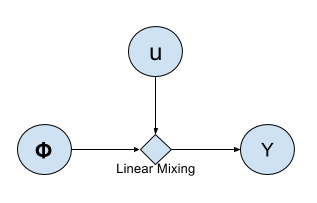
\includegraphics[scale=0.5]{images/GPFA_graphical_model.png}
    \caption{Graphical representation of GP based factor analysis model}
    \label{fig:gpfa_graph}
\end{wrapfigure}

Mathematically, model is very similar to the standard factor model described in previous section with the distinction that here latent factors $u$ are assumed to be conditionally independent GP, indexed through a common index $x$. As can be observed from Figure \ref{fig:gpfa_graph}, flow of information from each observed response to every latent factor response makes the sharing of statistical strength among response variables possible, thereby resulting in a much more expressive model than traditional factor analysis models. 
\newpage

The model is shown in figure \ref{fig:gpfa_graph} and can be expressed as,
\begin{equation}
Y=\phi u + \sigma^2I
\end{equation}

where ${u \in R^{P \times N}}$ are the latent factors that get linearly mixed through matrix  ${\phi \in R^{C \times P},}$ resulting in the observations ${Y \in R^{C \times N}}$. As in [Seeger], factor analysis emerges when $P << C $ 

We put a GP prior on latent variables $ u_p \in GP(0,K^p)$ where $K^p$ is the co-variance kernel for that particular Gaussian process. Loading matrix $\phi$ is assumed to have a Gaussian prior $N(0,I)$. 

\subsubsection{Variational Sparse Approximation of GPFA posterior}

To achieve sparsity in posterior, we approximate the posterior distribution as $ q(\phi,u,\hat{u})$ where  $p(\hat{u})$ is the distribution through n inducing points ( n << N). Finally, a GP prior is put on $p(\hat{u})$ too and the sparse approximation of posterior to factorizes as: 
\begin{equation}
q(\phi,u,\hat{u}) = q(\phi)\prod_{p=1}^{P}p(u_p \mid \hat{u_p})q(u_p)
\end{equation}

Based on above sparse approximation, marginal likelihood of data can be given as,
\begin{equation}
L(Y|X) = \int p(Y \mid \hat{u},\phi) p(\phi,\hat{u},u) d\phi du d\hat{u}
\label{eqn:gpfa_lklihd}
\end{equation}

Following the VB inference scheme as outlined in section 3, we find optimal distributions by minimizing the KL divergence between approximation and true posterior. This in turn is equivalent to maximizing the log of marginal likelihood given in equation \ref{eqn:gpfa_lklihd} with respect to each parameter(detailed derivations are given in Appendix 1) :

For $\hat{u_p}$, 
$${q(\hat{u}_p) \approx \mathcal{N}(\hat{u}_p \mid \Sigma_{p}^{-1}K_{nn}^{-1}K_{Nn}Z_p,\Sigma_{p}^{-1})
}$$
where, ${
\Sigma_{p} = K_{nn}^{-1} + \frac{1}{\sigma^2}K_{nn}^{-1}K_{nN}S_pK_{Nn}K_{nn}^{-1}}$ and 
${Z_p = \sum_{c}^{C}\mathbb{E}[\phi_{cp}](y_c - \sum_{i}^{P/p}\mathbb{E}[\phi_{ci}]\mathbb{E}[u_{ip}])}$.   

Similarly VB update for $\hat{\phi}$ can be derived as, 
$${q(\phi) \approx \mathcal{N}(\phi \mid y\mathbb{E}[U]^T\Sigma_{\phi}^{-1}, \Sigma_{\phi})}$$
where ${\Sigma_{\phi} = (V_{\phi}^{-1} + I )^{-1}}$
and ${V_{\phi} = \mathbb{E}[u]\mathbb{E}[u]^T\sigma^2}$

Finally update for ${u}$ is,
$${
q(u_p) \approx \mathcal{N}(u_p \mid M\hat{\mu_{p}}, \Sigma_{u \mid \hat{u}}^{p} + M\Sigma_pM^T)
}$$
where ${\hat{\mu_{p}}$ is the mean of GP $u_p$, ${M = K_{Nn}K_{nn}^{-1} }$ and
${\Sigma_{u\mid\hat{u}}^{p} = K_{NN} - MK_{nN} }$

\subsubsection{Hyper-parameter selection}
Hyperparameters for GP based FA that might require tuning mostly include the parameters for covariance kernel function of GPs corresponding to the latent factors. These can be optimized  by maximizing the marginal log likelihood with respect to the latent factors as:
\begin{equation}
L(\theta_p) = log \mathcal{N}(S_{p}^{-1}z_p \mid 0,S_{p}^{-1} + K_{Nn}K_{nn}^{-1}K_{nN}) - \frac{1}{2}tr(\sum_{i=1}^{P}S_{i}*cov(u_i \mid \hat{u}_i)) ) + consts.
\label{eqn:gpfa_likl_opt}
\end{equation}
where $S_p = \sum_{c}^{C}\mathbb{E}[\phi_{cp}^2]$

Using above equation one can obtain the gradients by differentiating the log likelihood corresponding to  each parameter $\theta_{p}$ of co-variance kernels associated with respective late factor GP. Recommended method of inference would be to first optimize hyperparameters and then find optimal distributions through VB updates while keeping the hyperparameters fixed. 

\subsubsection{Demonstrations on artificial data set}
\begin{figure}
    \centering
    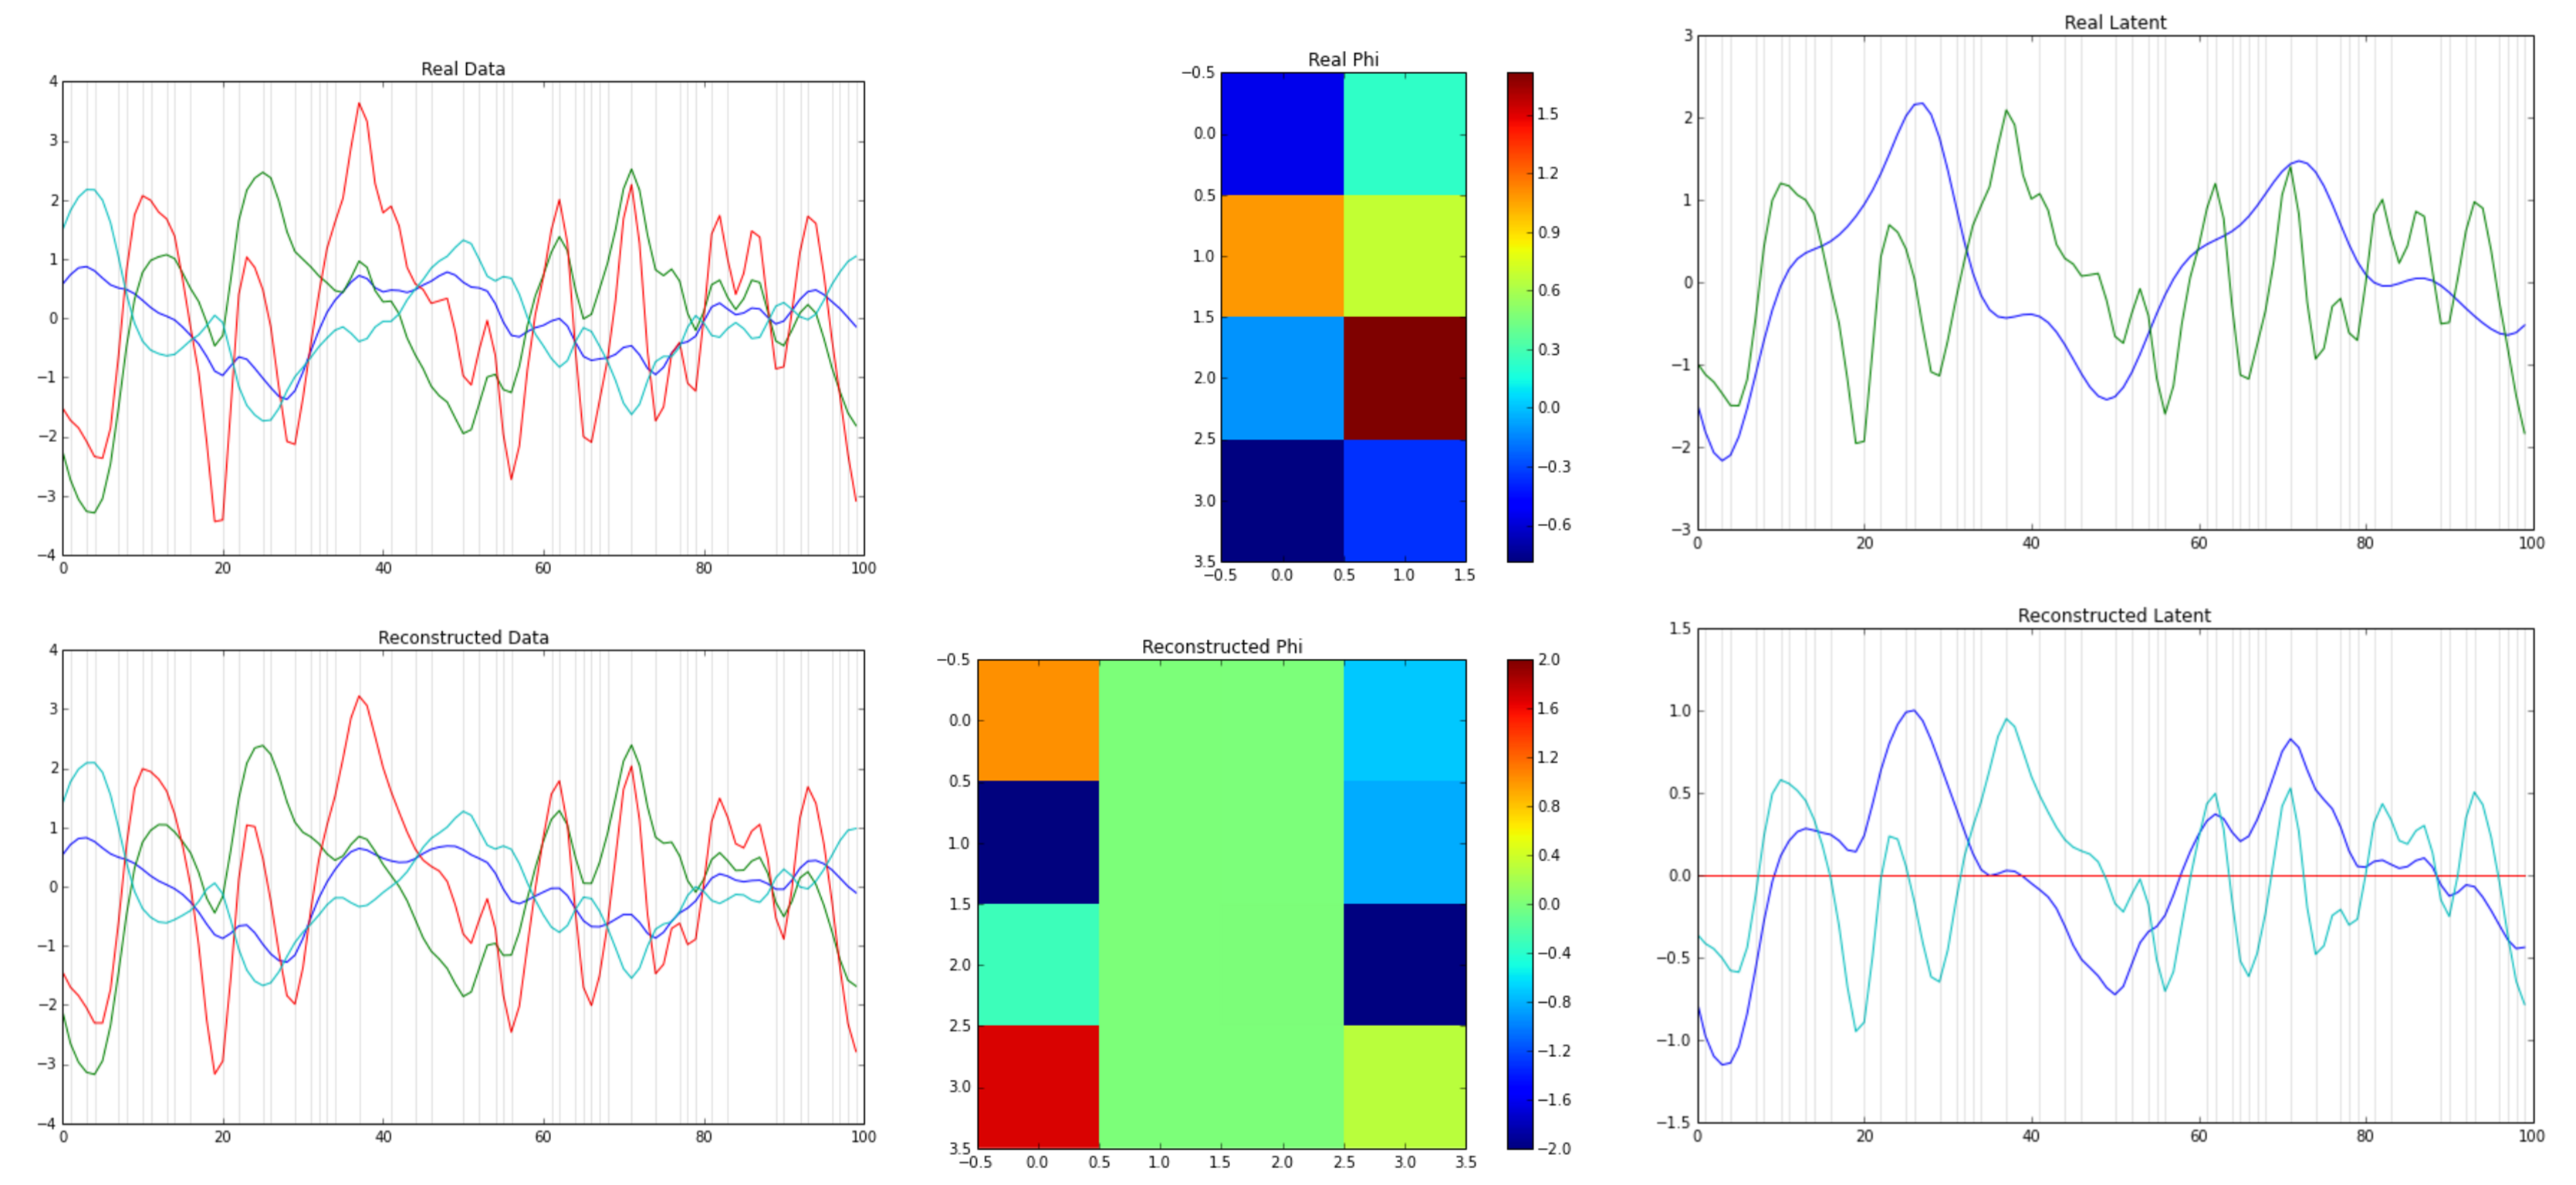
\includegraphics[scale=0.25]{thesis/images/SLFM_demo1.png}
    \caption{Extracting latent processes from artificial data set using GPFA: Upper row shows the real latent process and mixing matrix. Second row demonstrates the extracted latent structure using variational inference. Gray Spikes indicate the inducing points at which functions were evaluated}
    \label{fig:slfm_demo1}
\end{figure}

In order to demonstrate model’s ability to recover latent processes that might have been used in data generation processes, We generated two artificial data sets using distinct latent process sets. 

First data set was created by mixing two latent processes (using 100 evaluation points) with the squared exponential kernel and using a randomly generated mixing matrix. We then initialized the variational algorithm with four random latent processes with SE of lengthscale and variance one. The inducing set $u_p$ was chosen to be only half of the original data set selected randomly. As can be seen in the Figure \ref{fig:slfm_demo1} , the model was not only able to recover the latent process structure very well but also shut off two redundant latent processes acting very similar to ARD prior [Reference?]. Since the variational approximation recovers complete distribution of the latent processes as well as the loading matrix, it is possible to augment these values with the confidence (something that’s not possible in SLFM for mixing matrix).

\begin{figure}
    \centering
    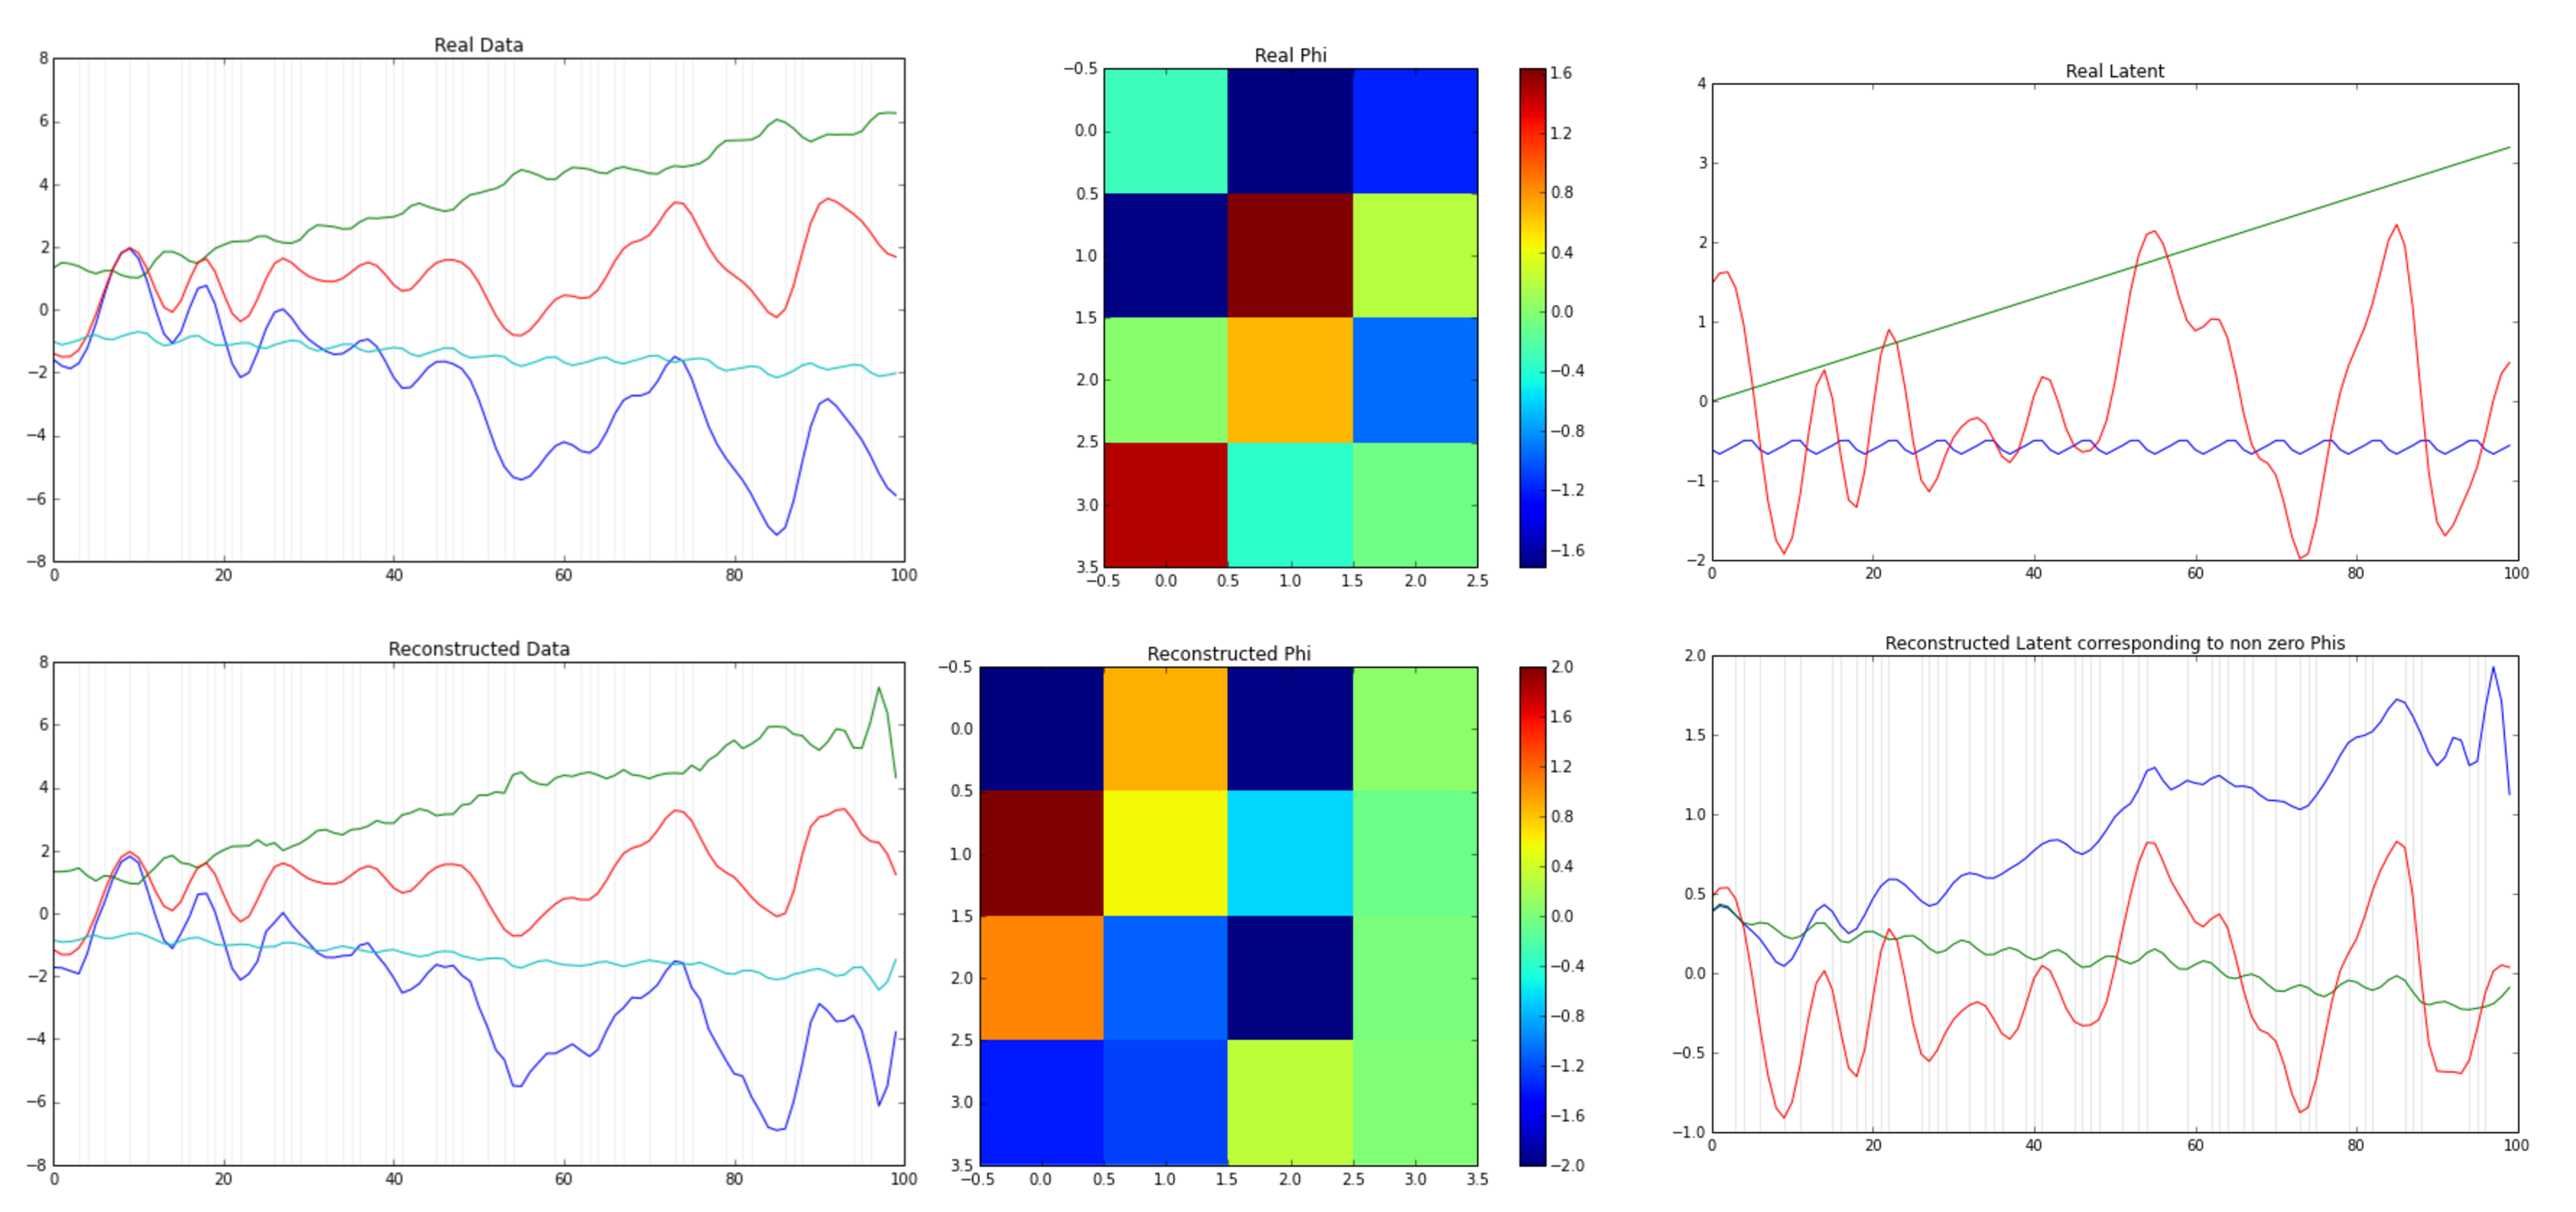
\includegraphics[scale=0.25]{thesis/images/SLFM_demo2.png}
    \caption{Extracting latent processes from artificial data set using GPFA: Upper row shows the real latent process (with periodic, linear and Gaussian kernels) and mixing matrix. Second row demonstrates the extracted latent structure using variational inference. Gray Spikes indicate the inducing points at which functions were evaluated}
    \label{fig:slfm_demo2}
\end{figure}

Since in most practical scenarios the latent process characteristics are unknown, an unsupervised model should be able to produce output that would be ultimately valuable to the user, i.e. would inform the user about characteristics of the dataset being analyzed. In this example, we generated data by mixing three different latent processes with the periodic, linear and Gaussian kernel using a randomly generated mixing matrix. To mimic the ignorance of analyst about data generating process we once again used four random Gaussian processes with only SE Kernels to initialize the inference algorithm. As can be seen from the results shown in Figure \ref{fig:slfm_demo2}, though imperfect, model is able to extract the cyclic and linear structures inherent in latent processes. Moreover, as in the previous example, model can automatically determine the redundancy and is able to shut off the extra latent process that we proposed in the beginning. 

\subsection{Extending GP based factor analysis}
Apart from the processes varying in time one of the main requirements in factor analysis is to support instance based scenarios, i.e. multiple instances with each instance having multiple response variables indexed by time. EEG data set [Sami's ref] is one of the prime example of the situation where each instance corresponds to a subject and variables include 50 second long readings of multiple sensors. The central motivation is to model scenarios where each instance can have its own specific inherent processes. 
Figure describes the model, now the output or observed data is considered to be in $S \times C \times N$ while $u$ in $S \times P \times N$ in where S represents the instances or trials and P latent factors. 
To accommodate multiple trials we fold Y and u in vectorized form i.e, 
$Y \in R^{S \times CN}, u \in R^{S \times PN }$ where $u \in GP(0,\bar{K})$ and $\bar{K}$ is  a block diagonal matrix of size PN x PN with covariance kernels ${K_p \in R ^{N \times N}}$ for each latent GP on it's diagonals, giving us follwoing generative model,
\begin{equation}
Y= u * \bar{\phi}^T + \sigma^2I
\end{equation}
${  \bar{\phi} = \phi \times I_{N \otimes N} }$ is also a block diagonal of size $CN \times PN$ with $C \times P$ matrix ${\phi}$ on its diagonal.

We apply the same procedure as in section 3.4 to find the posterior 

\subsubsection{ Approximations for Extended GPBFA }
Following the same procedure and notation as for the GP based factor analysis the sparse variational approximation for the extended format of GPFA can be given as,

For sparse distribution ${\hat{u}}$,
$${
q(\hat{u}_p) \propto N(\hat{u}_p \mid y\mathbb{E}[\phi]{K}_{pNpn}K_{pnpn}^{-1}\hat{\Sigma}_{u}^{-1}, \hat{\Sigma}_{u}^{-1})
}$$

where $\hat{\Sigma}_u = K_{pnpn}^{-1} + \frac{1}{\sigma^2}K_{pnpn}^{-1}K_{pnpN}F_uK_{pNpn}K_{pn}^{-1}$, $F_u = \mathbb{E}[{\bar{\phi}}^T{\bar{\phi}}] = Var({\bar{\phi}}) + \mathbb{E}[{\bar{\phi}}]^T\mathbb{E}[{\bar{\phi}}]$.

Similar to earlier section $u$ can be obtained as, 
$${
q(u_p) \propto N (\hat{\mu}_p M, \Sigma_{u_p|u^{p}} + M\Sigma_{u}M^{T})
}$$
where  $\hat{\mu}_{u}$ is the mean and ${\hat{\Sigma}_{u}}$ variance of $\hat{u}$, $\Sigma_{u|u^{p}} = K_{pNpN} - K_{pNpn}K_{pnpn}^{-1}K_{pnpN}$ and $M K_{pnpn}^{-1}K_{pNpn}$.

$\phi$ can be obtained as, 
$${\phi = N(\phi| (\bar{V}_{\phi} + I)^{-1}\bar{z}_{\phi}, (\bar{V}_{\phi} + I)^{-1})}$$
where $\bar{V}_{\phi} = \sum_{s}^{S}(<\bar{u}_s><\bar{u}_s>^T$ + I)
and $\bar{z}_{\phi} = \sum_{s}^{S}<\bar{u}_s>\bar{y}_{s}^T$
here $x = vec(\bar{x})$.

\subsubsection{ Demonstration of extended GPBFA}
\begin{figure}
    \centering
    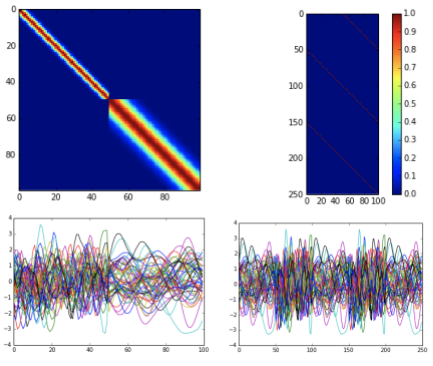
\includegraphics[scale=0.45]{thesis/images/eslfm_data.png}
    \caption{Artificial data set generated for Extended GPBFA: Upper row shows the SE Kernel for latent GP (with shorter and longer length scales) and mixing matrix. Second row demonstrates the actual latent GPs and resulting data generated by mixing them. }
    \label{fig:eslfm_data}
\end{figure}
To demonstrate the ability of extended GPBFA to extract different latent processes inherent in each instance we use an artificially generated dataset in which each instant is obtained by mixing two GPs (Figure \ref{fig:eslfm_data}). For identification purposes  we make one latent GP to have significantly shorter length scale than the other.
\begin{figure}
    \centering
    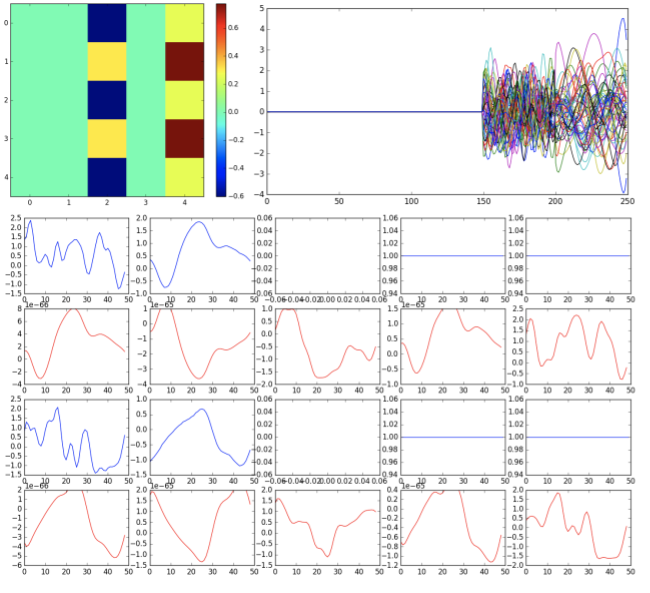
\includegraphics[scale=0.45]{thesis/images/eslfm_demo.png}
    \caption{Extracting latent processes using extended GPBFA: Upper row shows the real latent process (with periodic, linear and Gaussian kernels) and mixing matrix. Second row demonstrates the extracted latent structure using variational inference. Gray Spikes indicate the inducing points at which functions were evaluated}
    \label{fig:eslfm_demo}
\end{figure}
GPs for inference algorithm are initialized randomly with constant lengthscale and random mixing matrix. Figure \ref{fig:eslfm_demo} shows the correctly inferred binary mixing matrix along with redundant processes shut off. We also display comparisons between the actual and inferred latent processes of two random instances in Figure.Please note that all the results were obtained by using only $80\%$ of the data points.


\subsection{Conclusions}
In this section we first reviewed probabilistic linear factor analysis models. The mdoel later described as GPBFA is very similar to [Seeger], however they use IVM framework for inference of latent processes and provide point estimate for mixing matrix. In our treatment  of GPBFA we derived a sparse variational approximation for latent processes which provide complete probability distributions for both latent processes as well as the mixing matrix. Moreover, our experiments with artificial data showed that it our sparse solution is able to recover latent structure by using only half of the actual data thereby making the proposed inference process more scalable and time efficient. [Luttinen's] has a similar approach but also puts a temporal structure on mixing matrix.We further extended the GPBFA model to include multi-trial/instance support and demonstrated that a sparse solution is still capable of recovering separate latent processes from each instance effectively. 




